\documentclass[10pt]{article}
\usepackage{fontspec}
\setmainfont{Times New Roman}
\newfontfamily{\headingfont}{Times New Roman}
\usepackage[utf8]{inputenc}
\usepackage{xcolor}
\usepackage{authblk}
\usepackage{graphicx}
\usepackage[a4paper, total={6in, 8in}]{geometry}
\usepackage{float}
\usepackage{natbib}
%\usepackage[T1]{fontenc}
\usepackage{nomencl}
\usepackage{titlesec}
\usepackage{amsmath}

\usepackage{mathptmx} % Size of equations:
\DeclareMathSizes{9.8}{17}{7}{7}
\DeclareMathSizes{10.0}{10}{6}{6}
\DeclareMathSizes{10.95}{10}{7}{7}   % For size 10 text
\DeclareMathSizes{11}{19}{13}{9}      % For size 11 text
\DeclareMathSizes{12}{20}{14}{10}     % For size 12 text


\usepackage[toc,page]{appendix}

\titleformat{\section}
  {\normalfont\fontsize{10}{10}\sffamily\bfseries}
  {\thesection}
  {1em}
  {}
\titleformat{\subsection}
  {\normalfont\fontsize{10}{10}\sffamily\bfseries}
  {\thesubsection}
  {1em}
  {}
  
\makenomenclature
% This will add the units
%----------------------------------------------
\newcommand{\nomunit}[1]{%
\renewcommand{\nomentryend}{\hspace*{\fill}#1}}
%----------------------------------------------

\usepackage[style=authoryear-ibid,backend=biber, maxnames=2]{biblatex}
%\usepackage[style=apa,backend=biber,maxnames=2]{biblatex}
%\usepackage[style=chicago-authordate,backend=biber]{biblatex}


\addbibresource{references.bib}% Syntax for version >= 1.2

\title{ A semi-empirical method for predicting roll damping based on large experimental tests regression}
\renewcommand\Authfont{\small}
\renewcommand\Affilfont{\small}
\author[1,2]{Martin Alexandersson}
\author[1]{Wengang Mao}
\author[1]{Jonas W Ringsberg}
\affil[1]{Dept. of Mechanics and Maritime Sciences, Chalmers University of Technology, 41296 Gothenburg, Sweden}
\affil[2]{SSPA Sweden AB, 41296 Gothenburg, Sweden}
\affil[ ]{\textit {maralex@chalmers.se}}
\date{}

\begin{document}
\begin{figure}
    \centering
    
\includegraphics[width=\columnwidth]{figures/ICSOS_logo.png}
\end{figure}

\maketitle
\thispagestyle{empty}

\vspace*{-0.5in}
{\footnotesize
\noindent\rule{\columnwidth}{0.4pt}
\section*{Abstract}
\label{se:abstract}
IMO, the International Maritime Organization, has in the second generation intact stability criteria \parencite{imo_finalization_2016} addressed the importance of ships having sufficient roll damping to avoid parametric roll and large roll motions in dead ship condition as well as excessive acceleration. Semi-empirical methods such as Ikeda’s method is widely used to predict roll damping for practical purposes, especially in the early design stage of ships where computational fluid dynamics or experimental model tests are not feasible options. Recent work has shown that the applicability and accuracy of Ikeda’s method for modern hull forms are somewhat uncertain which is very unfortunate, especially for analysis of parametric roll. A small error in the roll damping prediction can make the difference between having no parametric roll and disaster \parencite{soder_ikeda_2019}.

The purpose of this work is to develop a new semi-empirical method to predict roll damping for modern ships. The method is developed with machine learning techniques applied on historical roll damping data. The data is obtained from roll decay model test conducted in the Maritime Dynamics Laboratory at SSPA Sweden AB (www.sspa.se) during the past 15 years. The method is meant to be used by the industry for practical purposes, where roll damping is used as input to various simulation tools. The accuracy can be estimated using cross validation, which is indeed very valuable information when the method is used in engineering applications. The method presented in this paper should, however, also be relevant for the research community where the possibilities of using machine learning on a large data base of high quality hydrodynamic data is explored. Improved roll damping predictions enables optimization for safer and more energy efficient ships. The new method is based on a large set of relatively new empirical data and should be more applicable to modern ships than older methods such as Ikeda’s method.

\noindent {\scriptsize \emph{Keywords}: Roll damping; Roll decay; Ikeda’s method; Simplified Ikeda’s method; Ship motions; Machine Learning}
}
\newline
\noindent\rule{\columnwidth}{0.4pt}
%\newpage
%\tableofcontents
%\newpage

\section{Introduction}
\label{se:introduction}

%\begin{itemize}
%    \item Roll damping important
%    \item Roll decay test at zero speed and %speed.
%    
%\end{itemize}
			
Ship roll has been the subject of several studies over the past decades. Roll damping devices include tuned liquid dampers such as anti-rolling tanks as well as exterior appendages such as bilge keels. Both passive and active anti-rolling devices have been investigated. Theoretical, numerical and experimental studies have been performed and presented in the literature. A classic example of an experimental study is presented by [1] for roll without forward speed. Different components of damping were studied in a series of publications by [2], [3] and [4]. Both naked hulls and hulls with bilge keels were
studied therein. Due to a significant amount of
experimental data for conventional hulls with bilge keels, for instance as presented in the above mentioned publications, good empirical formulas have existed for several decades. The report by Himeno (1981) presents a comprehensive summary of the state-of-the-art at that time, and formulas presented therein are still used today IMO (2016).

The computer power and availability of fast, stable NaviérStokes solvers have made it feasible to a larger degree to study the problem numerically in recent years, and this trend is expected to continue. However, having model tests as benchmark data will remain a requirement. The experiemental methods and semi-empirical formulas are still in a great demand espeically in the ship conceptual design and inspections, see IMO (2016). In this paper we present results from experiments and semi-empirical method proposed by Ikeda\'s method of a big database towing tank tests from SSPA. In order to faciliate the usage of the SSPA roll-decay test basebase, the Ikeda\'s method is further developed to reflect the state-of-the-art ship design with correct roll damping properties. 


%
%\fbox{\begin{minipage}{40em}
%    {\footnotesize
%        \mbox{}

\printnomenclature
%    }
%\end{minipage}}

\section{Methods for prediction and analysis of roll damping}
\label{se:methods_for_prediction_and_analysis}

\subsection{Hydrodynamics}
\label{se:hydrodynamics}
The roll damping consists of linear and nonlinear components. At zero speed the nonlinear damping is caused by the two-dimensional separation at the bilge keel or near the bilge circle (Eddy damping $B_E$). While at speed the nonlinear damping is mainly caused by the hydrodynamic lift force on the hull, represented as lift damping $B_L$. $B_E$ vanishes at high speed ($F_n>0.15)$ \cite{ikeda_components_1978}.

The wave damping also changes at speed. Ikeda \cite{ikeda_components_1978} proposes a formula for the fraction between wave damping at speed and zero speed: $\frac{B_W}{B_{W0}}$

The Ikeda method has been used to calculate the roll damping for a PCTC vessel Faust \cite{soder_assessment_2019}.
\begin{figure}[h]
    \centering
    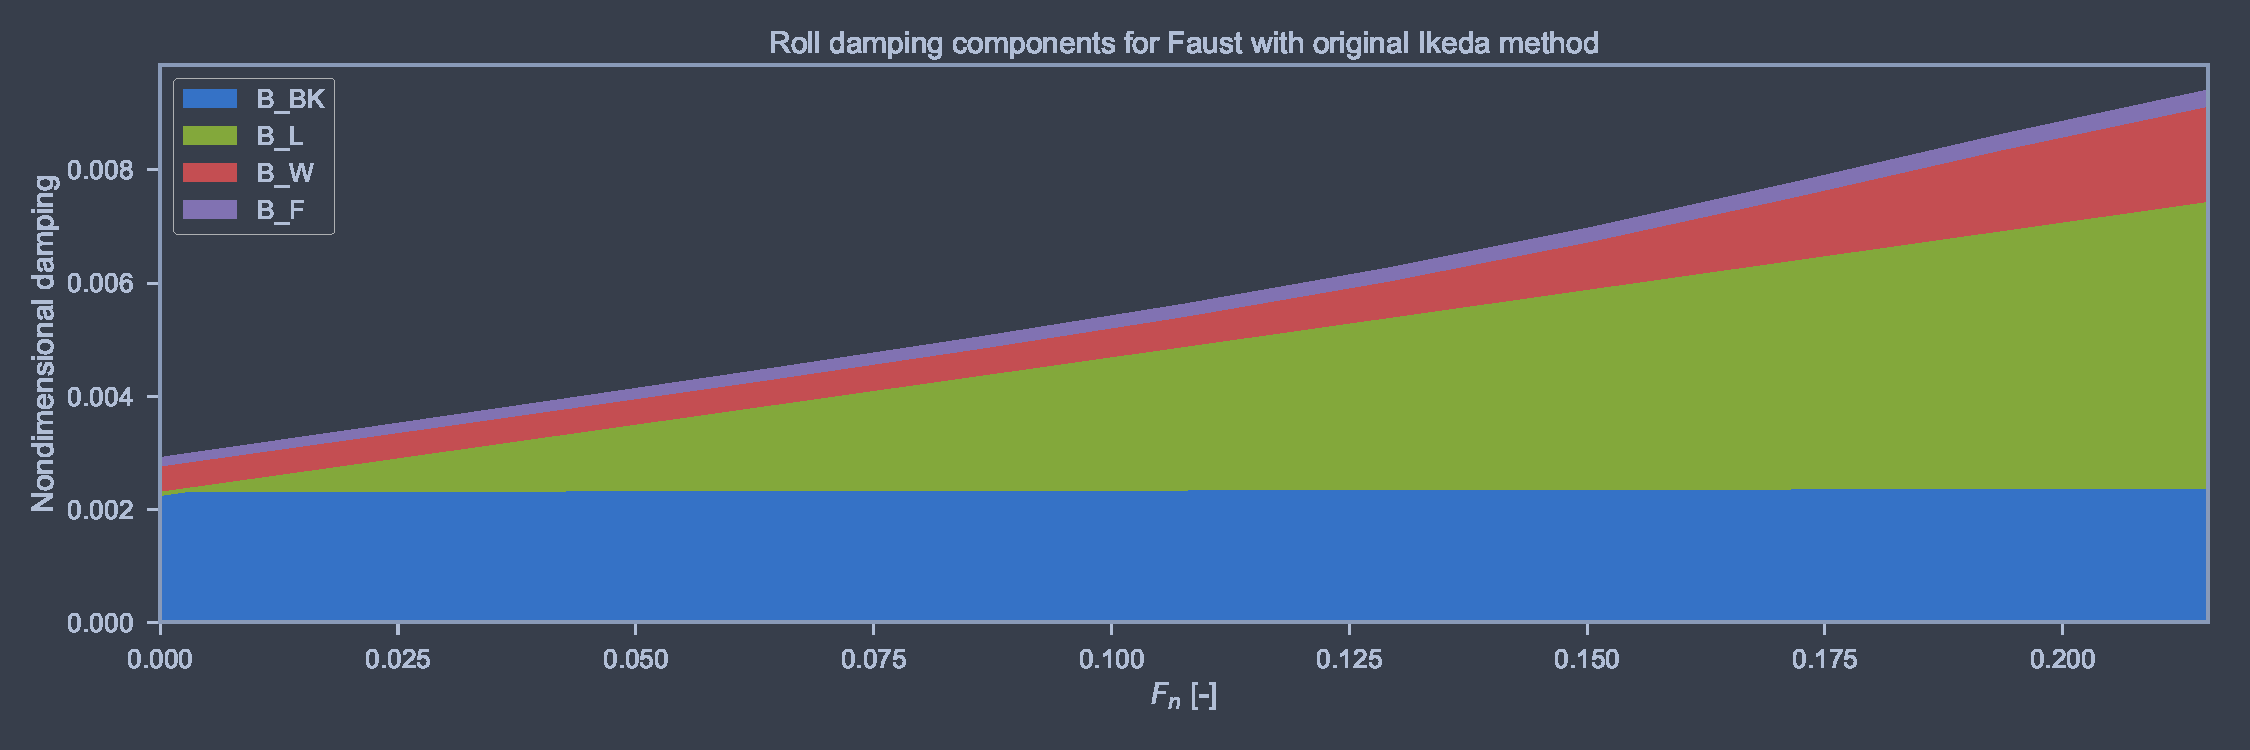
\includegraphics[width=\columnwidth]{figures/ikeda_faust.pdf}
    \caption{Roll damping components calculated with Ikeda method for PCTC Faust}
    \label{fig:ikeda_faust}
\end{figure}



Ikedas original method require strip method calculations. This is not an attractive option for the present study since that would require calculations with exact hull geometries to be carried out for all of the ships in the study. There exist however a \emph{Simplified Ikeda method} \cite{kawahara_simple_2011} that is instead used in this study \emph{Simplified Ikeda method} predicts the roll damping components at zero speed.

A study of the has been conducted which shows the roll damping components for various speeds. Calculations with *Ikeda original method* and the *Simplified method* have been carried for two ships (*S175* and *Faust*). The two methods show reasonable agreement for zero speed.

In order to introduce a speed dependancy to the *Simplified method* the following is conducted:
* Add Lift damping $B_L$.
* Add speed dependence of wave damping $\frac{B_W}{B_{W0}}$
* Remove $B_E$ at ($F_n>0.15$) ?
\section{Accuracy of current methods for predicting roll damping}
\label{se:accuracy_SI_method}
It was shown by \parencite{kawahara_simple_2011} that Ikeda's method does not work for some modern ships with buttock flow sterns. \parencite{soder_assessment_2019} also showed that Ikeda's method was not capable of accurately predicting the roll damping for a Pure Car and Truck Carrier. The SI-method being a simplified version of Ikeda's method most likely inherits its problems but also introduces some extrapolation errors as reported by \parencite{rudakovic_application_2017}. In the following, 227 existing roll decay model tests conducted at SSPA Maritime Dynamics Laboratory are used to validate the SI-method. The comparison will help identify the drawbacks and improvement potentials of the SI-method. It aims at further developing this method to increase its accuracy through some statistical regression analysis based on the large test database.

\subsection{Overall accuracy of Simplified Ikeda method}
\label{se:overall_comparison}
%An investigation of how well the implementation of the SI-method agrees with the corresponding results in the roll damping database has been carried out. 
Comparing roll damping is a bit difficult since the roll damping model consist of two coefficients, a linear term $B_1$ and a quadratic term $B_2$. These coefficients can be combined by calculating the equivalent damping coefficient for a certain roll angle $\phi_a$ \parencite{himeno_prediction_1981}:

\begin{equation}
B_{e} = B_{1} + \frac{8 B_{2} \omega_{0} \phi_{a}}{3 \pi}
\end{equation}


For the roll damping database $B_1$ and $B_2$ can be inserted directly into Eq.(\ref{eq:B_e_equation}) to get the equivalent roll damping $B_e$. In order to obtain the same coefficients for the SI-method, roll damping was calculated for two roll amplitudes $\phi_a$ for the same motion frequency. $B_1$ and $B_2$ are obtained by fitting the Eq.(\ref{eq:B_e_equation}) to this data \parencite{himeno_prediction_1981}. The $B_e$ coefficient was made non-dimensional according to \parencite{himeno_prediction_1981}  giving the non-dimensional equivalent linear damping coefficient $\hat{B_e}$, which was more convenient to use for this comparison as follows,
\begin{equation} \label{eq:be_eqvalent}
    \hat{B_e} = \frac{B_e}{\rho \bigtriangledown Beam^2} \sqrt{\frac{Beam}{2g}},
\end{equation}
where $\rho$, $\bigtriangledown$ and $Beam$ stand for fluid density, displacement volume and breadth of a ship, respectively.
For the roll decay tests at SSPA, i.e., the database used in this study, the initial roll angle is normally set to 10 degrees, so that the model test data contain amplitudes in the range between 0 and 10 degrees. The root mean squared error of the equivalent roll damping, $RMSE_{\hat{B}_e}$, for various initial roll angles $\hat{B}_e(\phi_a)$ between estimation by the SI-method and the model test results is,

\begin{equation} \label{eq:rmse}
    RMSE({\hat{B}_e} (\phi_a)) = \sqrt{\frac{\sum\limits_{i=1}^n (\hat{B}_{e,i}^{SI} (\phi_a) - \hat{B}_{e,i}^{model} (\phi_a))^2}{n}},
\end{equation}
where $\hat{B}_{e,i}^{SI} (\phi_a)$ represents the equivalent roll damping by the SI-method for the i-th model test with initial roll angle of $\phi_a$, while $\hat{B}_{e,i}^{model} (\phi_a)$ represents the damping from the model tests. The results of the RMSE are plotted in the upper plot of Fig.\ref{fig:ikeda_phi_a}. Large values of $RMSE({\hat{B}_e})$ indicate very bad agreement between the SI-method and the model test results for roll damping prediction of modern ships. It should be noted that the accuracy decrease for larger amplitudes where nonlinear part of the SI-method plays a larger part. Furthermore, in order to illustrate the difference of $\hat{B}_e$ prediction between the SI-method and the model tests at SSPA, the three bottom plots of Fig.\ref{fig:ikeda_phi_a} presents the comparison for three roll amplitudes $\phi_a$ equal to 0, 5, 10 degrees, respectively. It shows that the accuracy differ very much between the amplitudes, with the highest accuracy at zero roll amplitude. 


\begin{figure}[H]
\centering
  \centering
  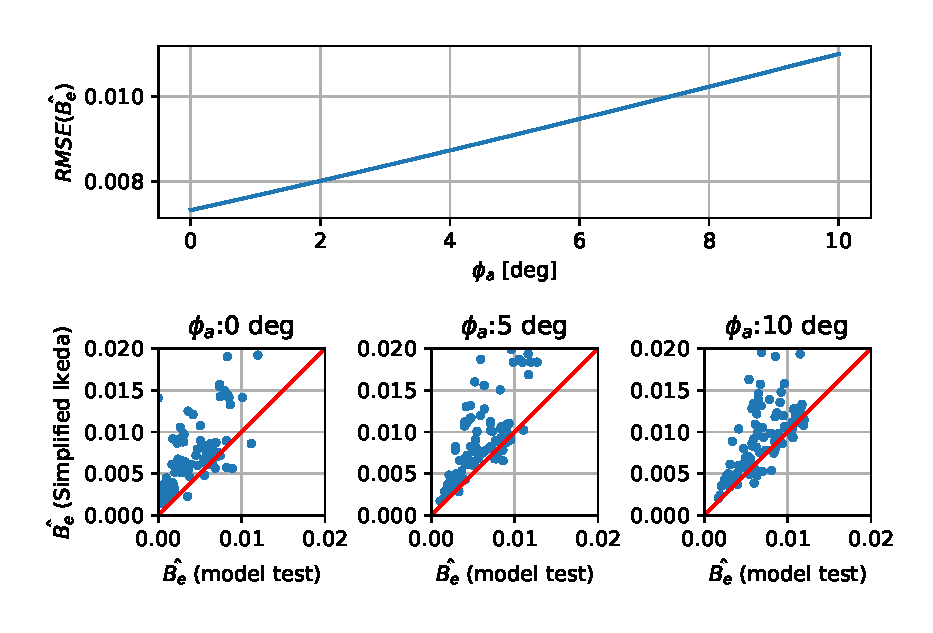
\includegraphics[]{figures/ikeda_phi_a.eps}
  \vspace{-0.5cm}
  \caption{Root mean square error of roll damping prediction between the SI-method and the model test results (upper plot). Influence of roll amplitude $\phi_a$ on $\hat{B_e}$ between the SI-method and model tests for $0^{\circ}$ (bottom left plot), $5^{\circ}$ (bottom middle plot) and $10^{\circ}$ (bottom right plot), respectively.}
  \label{fig:ikeda_phi_a}
\end{figure}

It was found that almost all ships in the roll damping database were outside the limits that are suitable to be applied in Eq.(\ref{eq:SI_limits}). Two different ways to handle this limit exceedance was investigated:
\begin{enumerate}
  \item the ``unlimited" approach where the input values are allowed to exceed the limits.
  \item the ``limited" approach where the limit boundary values were used for exceeding values.
\end{enumerate}

Fig.\ref{fig:ikeda_limited} show the comparison of roll damping predictions by the SI-method at 2 degrees roll amplitude, using the ``unlimited" and ``limited" approach with the corresponding results from model tests. The ``limited" approach seems to be the best one to use according to this figure, where the ``unlimited" approach has values very far away from the model test results (far away from the red reference line).   


\begin{figure}[H]
\vspace{-0.5cm}
\centering
  \centering
  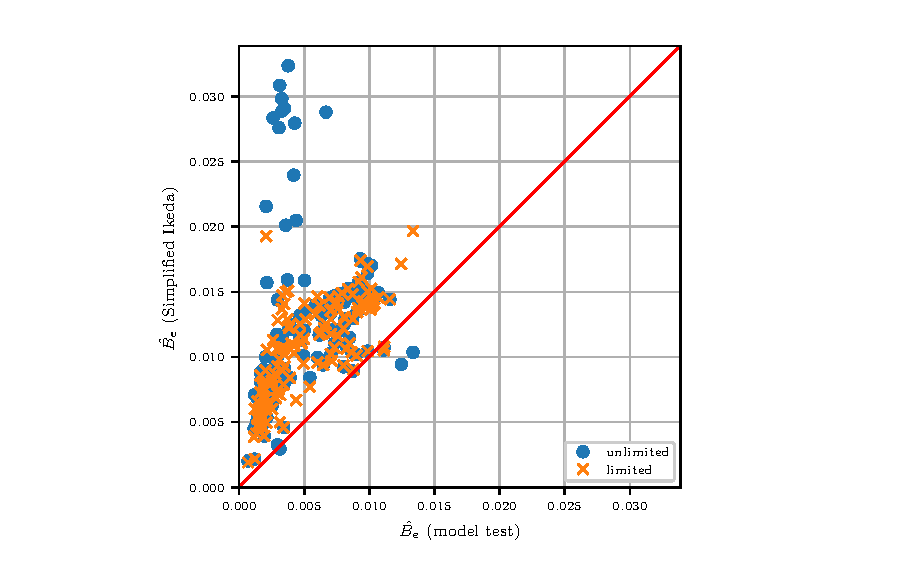
\includegraphics[]{figures/ikeda_limited.eps}
  \vspace{-0.5cm}
  \caption{$\hat{B_e}$ at all speeds estimated by the simplified Ikeda's method (Y-axis) in comparison with that from the roll decay test database (X-axis)}
  \label{fig:ikeda_limited}
\end{figure}


\subsection{Sensitive analysis of SI methods for the ship data}
\label{se:accuracy_SI_method}
Prior to the validation the behaviour of the SI-method was studied by varying the input parameters between minimum and maximum values in database around a point "reference ship" with values in the middle of the input boundaries (Eq. \ref{eq:SI_limits}) (see figure \ref{fig:SI_sensitivity}). It can be seen that the wave damping $B_W$ increases a lot with the absolute value of $OG/T$. It can also be seen the the wave damping has an enormous increase when the beam to draught ratio exceeds the input boundary, which seems to be the case for at least one third of the roll decay tests. It can also be noted that most of the ships in the database have midsection coefficients $A_0$ and bilge keel heights outside the limits. 

\begin{figure}[H]
    \centering
    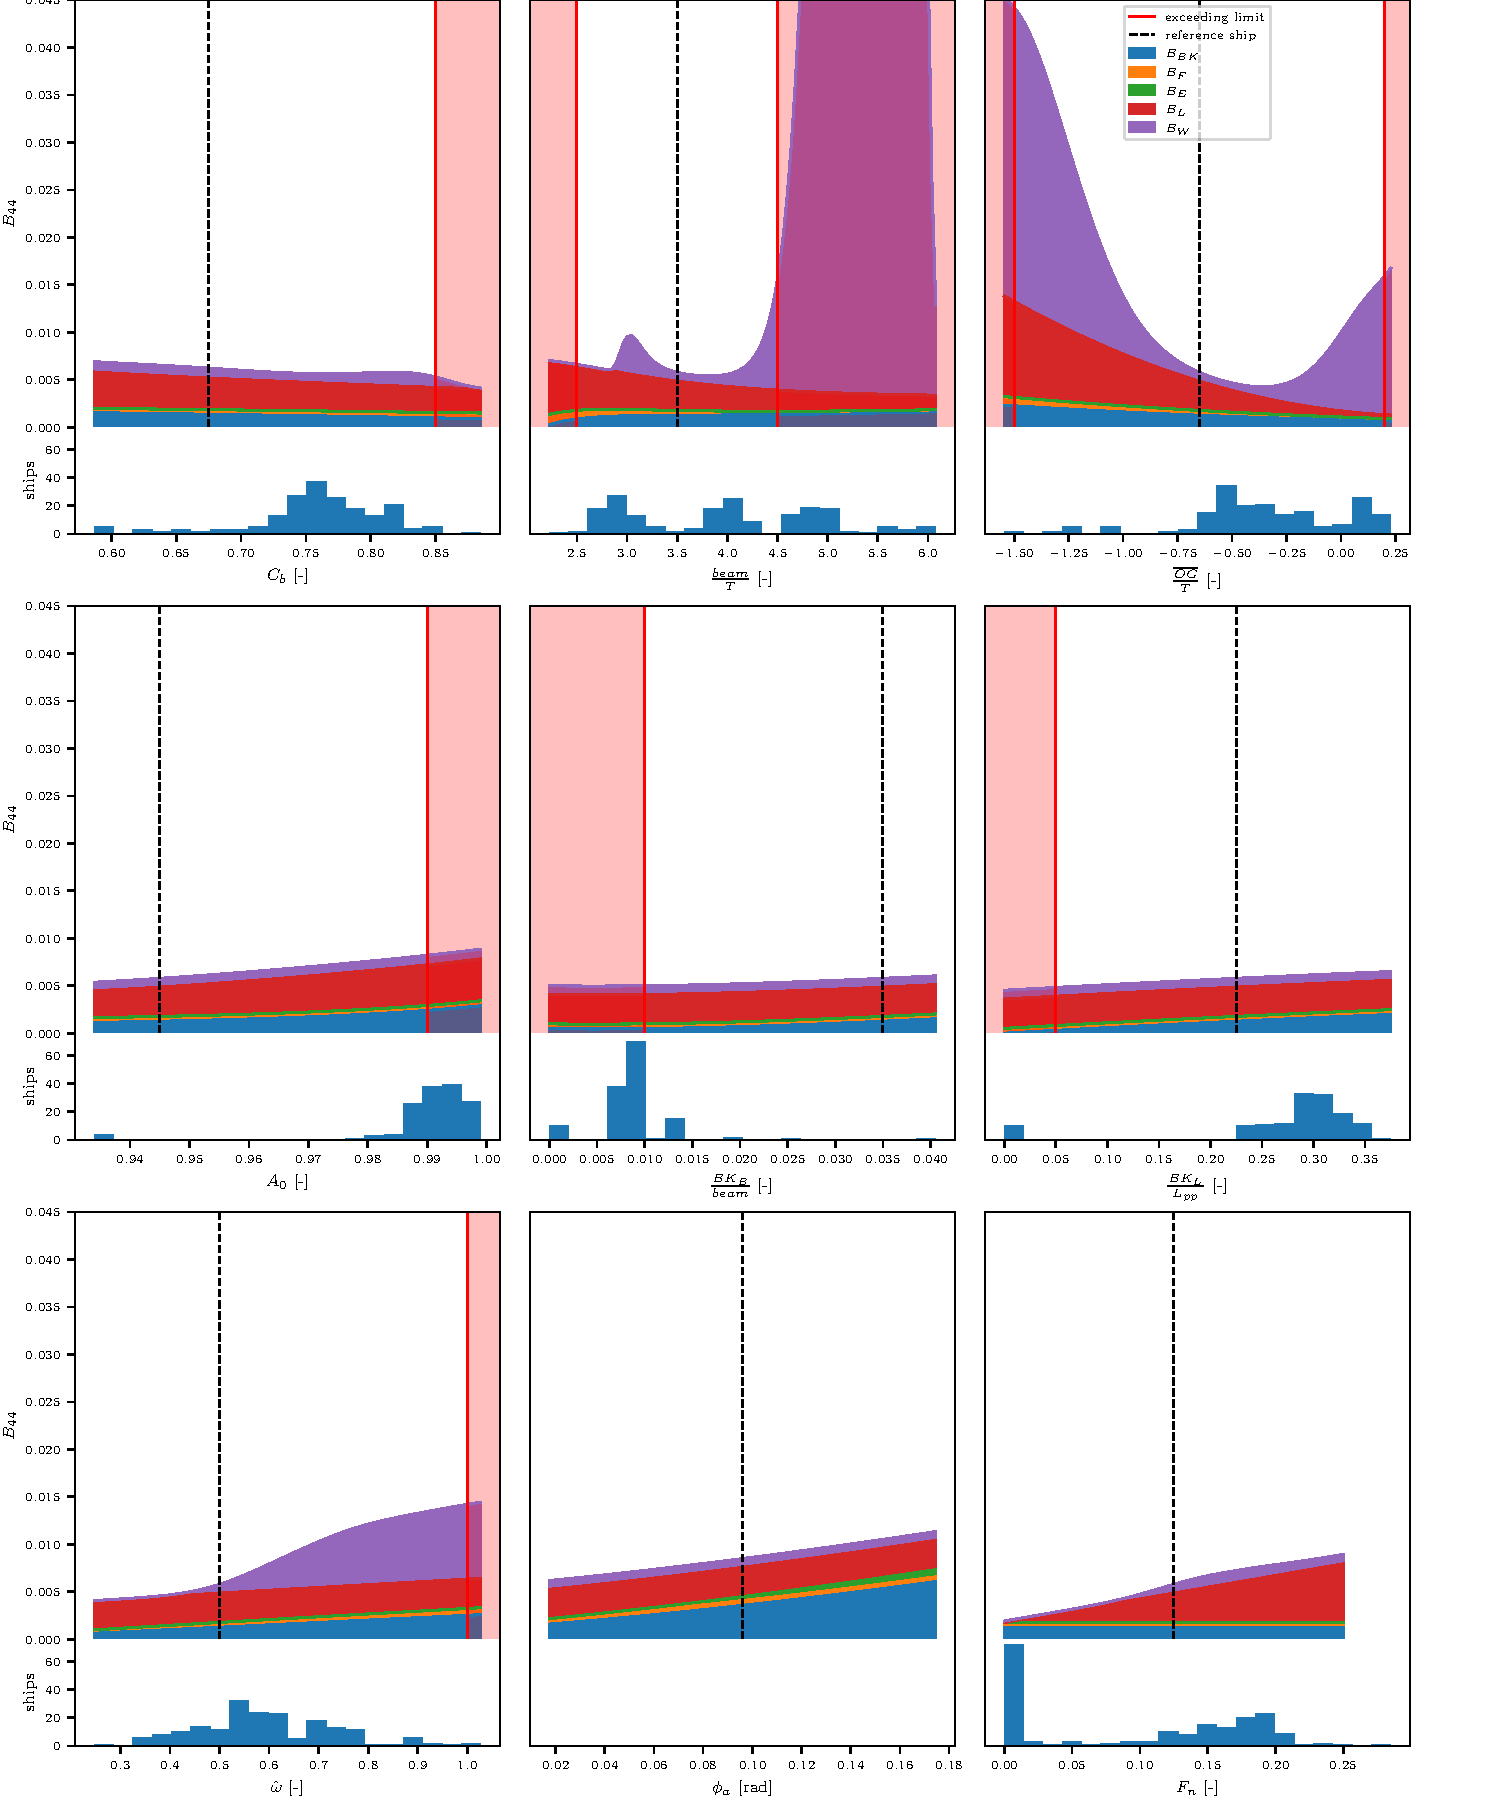
\includegraphics[width=\textwidth]{figures/SI-sensitivity.pdf}
        \vspace{-0.5cm}
    \caption{SI-method input parameter variation and data base ships}
    \label{fig:SI_sensitivity}
\end{figure}


\subsection{Simplified and original Ikeda method}
\label{se:si_ikeda_model}
Since the agreement between the SI-method and the reference model test result was not very good a second study was conducted to see if the original Ikeda method would give better results. In the Ikeda method more detailed information about the ship hull geometry is needed so that $B_W$ can be calculated with a strip method and $B_E$ can be calculated using sectional lewis coefficients. It was possible to collect the required hull inputs for 14 ships in the database. Scale models of these ships were used in 46 of the reference roll decay tests.

\begin{figure}[H]
    \centering
    \includegraphics[width=6in, height = 8in ]{figures/si_}
        \vspace{-0.5cm}
    \caption{SI-method input parameter variation and data base ships}
    \label{fig:s}
\end{figure}

\section{Regression method based on SSPA database}
\label{se:correction_SI_method}
In order to improve the accuracy of the roll damping prediction, the SSPA database containing more than 250 roll decay tests with modern ships is used to propose new models. In the following preliminary investigation, two different approaches are used to build such a model for roll damping prediction. The model is assumed to be a function of the same input parameters as the SI-method (see Eq.(\ref{eq:S1-method})). It was found in section \ref{se:overall_comparison} that the $B_e$ coefficient changes a lot with the roll amplitude $\phi_a$ which introduces a challenge to this regression. Three different options to approach this were considered:
\begin{itemize}
    \item Calculate $B_e$ for only one representative value of $\phi_a$.
    \item Split the problem into two regressions, one for $B_1$ and one for $B_2$.
    \item Calculate $B_e$ for a range of $\phi_a$ and include all in the regression.
\end{itemize}
The first option was rejected because that would generate a model that works for one roll amplitude only. The second option was rejected because introducing two regression models was considered unnecessary complex. And it was also suspected that there could be correlations between $B_1$ and $B_2$ so that the two regressions needed to be connected in some way. So the third option was used which means that the $B_e$ used in the regression contains roll amplitudes between 0 and 10 degrees.  

\subsection{New regression model for roll damping}
The first approach assumes that the function can be expressed as a second order polynomial. Some statistical learning method is used to establish the regression model. The input parameters (the features) are first transformed into polynomial features including all possible coupling terms. The best polynomial features are selected using a feature selection algorithm, selecting the k-best features \parencite[]{noauthor_sklearnfeature_selectionselectkbest_nodate} with a linear model for testing the individual effect of each feature \parencite[]{noauthor_sklearnfeature_selectionf_regression_nodate}. 

Cross validation, as described in section \ref{se:cross_validation} below, is used to estimate the accuracy. The optimum number of polynomial features was determined by finding the "k-value" with the highest accuracy in the cross validation. A regression model with 12 polynomial features was found to have the best accuracy when evaluated in this way. The model was determined by fitting the selected regression model to the entire data, giving the following expression:

\begin{equation} \label{eq:polynom_complex}
\begin{aligned} 
 \hat{B_{e}} = - 0.02578 A_{0} V - 0.02705 BK_{B} V + \\ 
 0.008993 BK_{L} V - 0.03191 C_{b} V - 0.2028 OG V + \\ 
 0.003472 V^{2} + \\ 
 0.004234 V \hat{\omega_{0}} - 0.008384 V beam - 0.002591 V phi_{a} + \\ 
 0.05048 V + \\ 
 0.007814 \hat{\omega_{0}}^{2} + \\ 
 0.03882 \hat{\omega_{0}} phi_{a} - 0.001069 \\ 
 \end{aligned}
\end{equation}

All the inputs with length scale ($T$, $B_{KB}, $B_{KL}$, $beam$) are nondimenilaized with $L_{pp}$. $V$ is nondimenionalized using $\sqrt{L_{pp}$. The middsection coefficients $A_0$ and block coefficients $C_b$ are nondimensional. The roll amplitude $\phi_a$ is in radians.


\subsection{Correction of Simplified Ikeda's method}
The second approach uses the SI-method as is, but then applies some corrections to the output damping components. A roll amplitude correction factor was also added. The correction factors was determined by fitting a linear regression model to the roll damping components giving the following expression: 
\begin{equation} \label{eq:polynom_correction}
\hat{B_e} = 1.106 \hat{B_BK_e} - 0.9124 \hat{B_E_e} + 4.282 \hat{B_F_e} + 0.7457 \hat{B_L_e} + 0.1844 \hat{B_W_e} + 0.004999 \phi_{a} - 0.0005097
\end{equation}

The proposed correction factors implies that $\hat{B_{BK}}$ and $\hat{B_{W}}$ should be reduced, $\hat{B_{E}}$ should be made negative and $\hat{B_{L}}$ does not need much correction.

A new semi empirical method to predict roll damping has been developed as an alternative or complement to the simplified Ikeda's method. The method  predicts roll damping as a simple mathematical expression based on main particulars and does not require a hull geometry definition. 
The new method is based on regression of the present roll damping database with some additional components of Ikeda's method. Since the underlying data is collected from roll decay tests, the methods predicts the roll damping at the natural frequency $\omega_0$.  
The regression was conducted on the roll damping database for tests at even keel. 

The roll damping database reveals that the roll damping at zero speed is much lower than the roll damping at speed. The hydrodynamics at zero speed and at speed is very  different \parencite{ikeda_velocity_1979}. These two situations need to be separated so that  the regression is formulated  as a product of two sub models:
\begin{equation} \label{eq:regression_factor_equation}
B_{e hat} = B_{e factor} B_{e hat 0}
\end{equation}

Where $B_{ehat0}$ is a zero speed regression and $B_{efactor}$ is a speed depending regression. A similar approach was used in \parencite{henry_peter_piehl_ship_2016}. Linear regression is  used for the two sub models. 

\subsection{Cross validation}
When constructing a regression model from a data set, over-fitting the data can be a problem. Including too many parameters and/or allowing too high order of the model would give a very good representation of the present roll damping data, but large extrapolation errors when the model is used on other data. Cross validation has been used to "mimic" this situation, where the model should make predictions on "new data", for ships that have not been part of the regression (the training of the model). The model that can make the best prediction on "new data" is considered as the best. The best model has been developed by optimizing the selection of parameters (the features). The regression model was allowed to have features selected from a "gross list" of all available meta data. The linear regression should determine coefficients in a mathematical expression represented as a polynomial up to second order and including coupling terms. The model with a selection of terms that gives the highest score in the cross validation is considered as the best.    

For the cross validation the data was divided into a  training set (80\%) and a testing set (20\%). The selection was made so that all tests with a specific ship model and its loading conditions were all in either the training set or the testing set. Only tests where there were results for both zero speed and speed (for the same loading condition and ship model) were included.

The "gross list" of available features has been chosen as a balance between guessed relevance and to minimize the number of tests that need to be excluded due to missing meta data. 
The number of parameters was also kept to a minimum so that a set of fewer features was selected prior to one with more features if they had similar scoring. As it turned out the developed regression models (equation \ref{eq:polynom_zero} and \ref{eq:polynom_speed}) have no coupling terms or quadratic terms.

The total regression model, consisting of the two sub models, was evaluated using cross validation. 100 random train/test sets were fitted and tested giving an average score: $mean(R^2)=0.68$, with standard deviation $std(R^2)=0.12$.

Figure \ref{fig:B_e_hat0_regression} and \ref{fig:B_e_factor_regression} shows comparisons between the regressions and the corresponding model test data. It can be noted that the speed factor can be up to 3.5 so that the roll damping at speed is 3.5 times larger than the corresponding roll damping at zero speed. The regressed sub models are shown in equation \ref{eq:polynom_zero} and \ref{eq:polynom_speed}. The non-dimensional damping due to hull lift $B_{LHAT}$, from the Ikeda method, is one of the parameters in the speed dependency equation \ref{eq:polynom_speed}. A comparison for the total regression model (equation \ref{eq:regression_factor_equation}) is shown in figure \ref{fig:B_e_factor_regression_total}, where it can be noticed that the error does not have the same ship draught dependence as the simplified method has. 

\begin{equation} \label{eq:polynom_zero}
B_{e hat} = - 0.0136052800165908 A_{0} + 0.759326775676605 BK_{B} + 0.0725876320147426 GM - 0.0303297720484823 T + 0.00126493893040265 \omega_{0 hat} + 0.0143189616219315
\end{equation}

\begin{equation} \label{eq:polynom_speed}
B_{e factor} = 84.1 B_{L HAT} + 3.64 V + 0.468
\end{equation}

{\footnotesize \underline{Note}: All input parameters are normalized using Froude scaling with $L_{pp}$ as scale factor. $\omega_{0hat}$ is non-dimensional according to \parencite{himeno_prediction_1981}.} 

\begin{figure}[H]
\centering
\begin{minipage}{.5\textwidth}
  \centering
  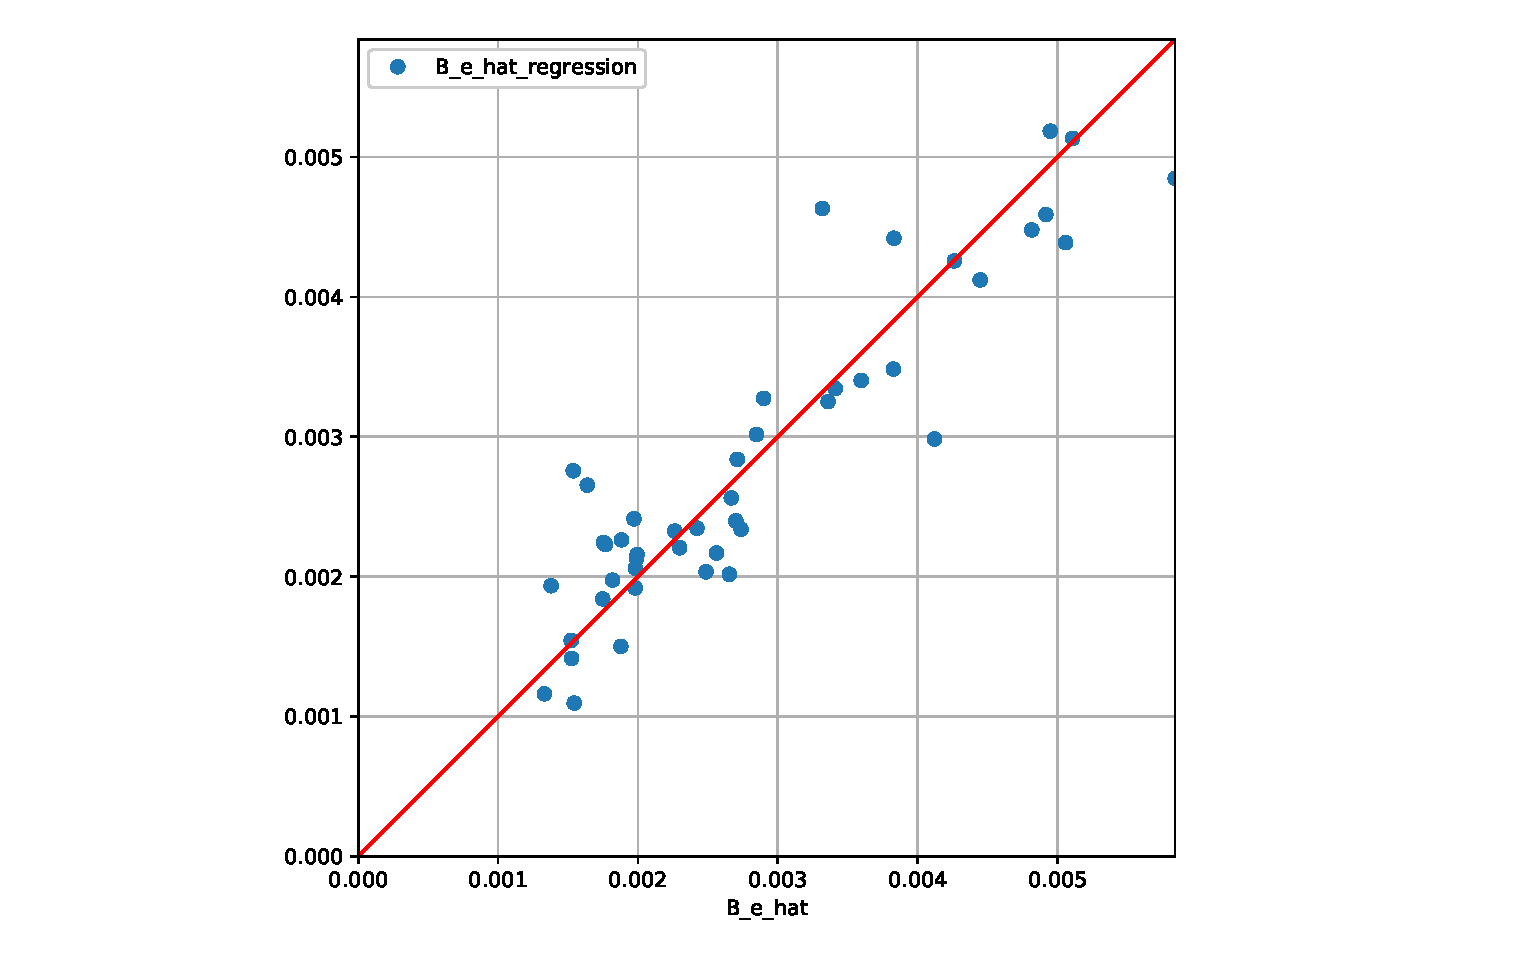
\includegraphics[width=\columnwidth]{figures/B_e_hat0_regression.eps}
    \caption{Comparison between predictions with the zero speed model and the damping at zero speed from the database}
    \label{fig:B_e_hat0_regression}
\end{minipage}%
\begin{minipage}{.5\textwidth}
  \centering
 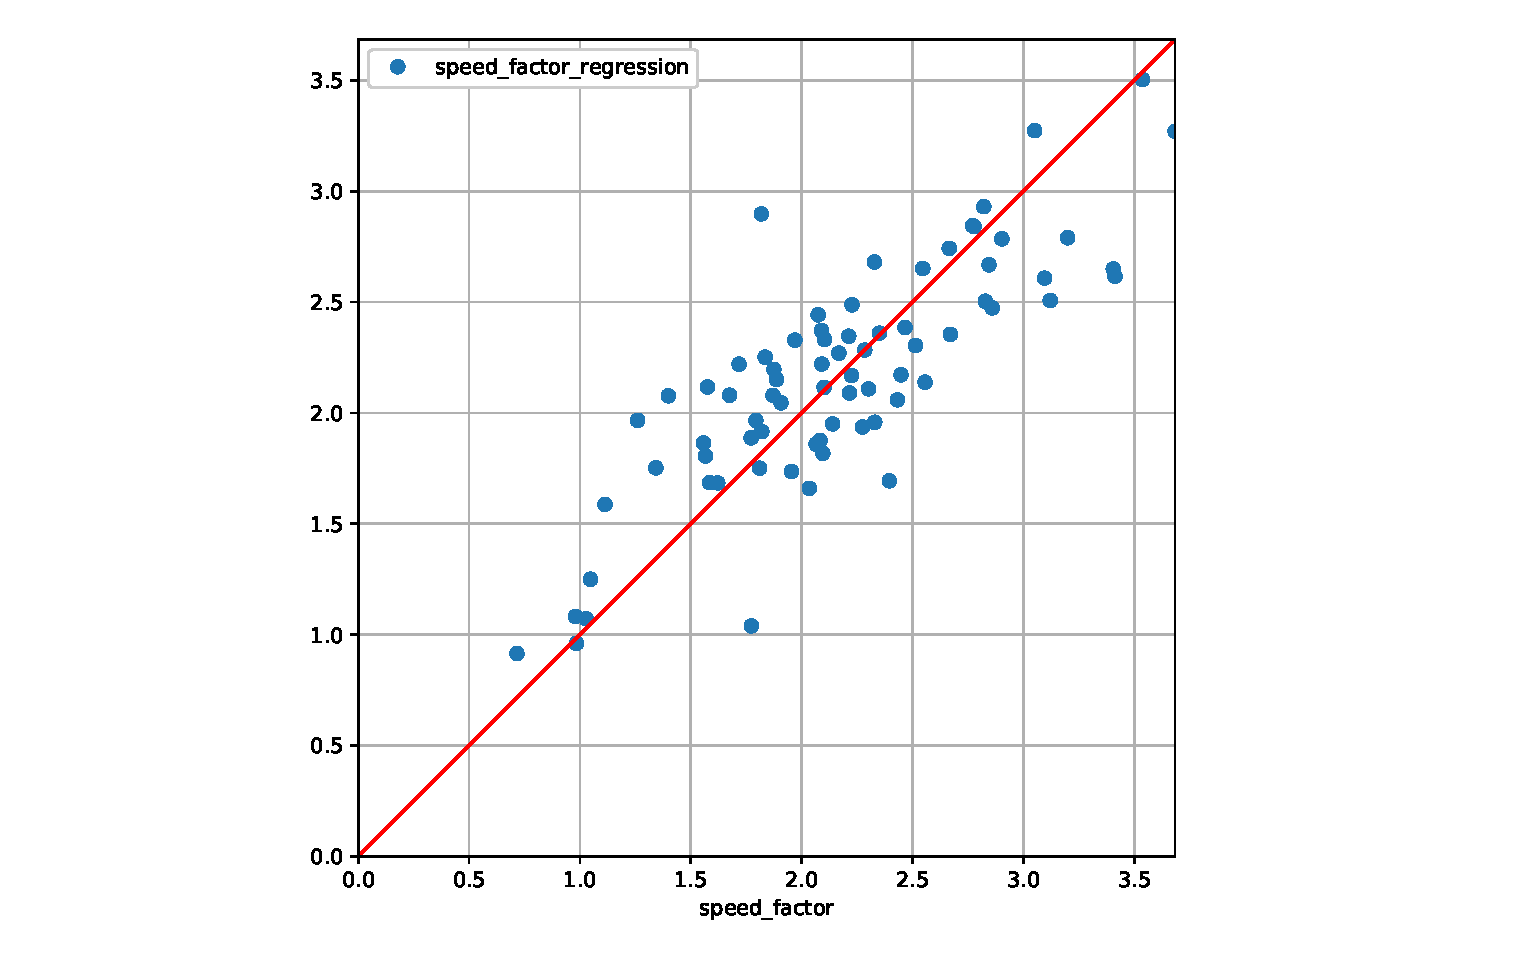
\includegraphics[width=\columnwidth]{figures/B_e_factor_regression.eps}
    \caption{Speed dependency regression}
    \label{fig:B_e_factor_regression}
\end{minipage}
\end{figure}


\begin{figure}[H]
    \centering
    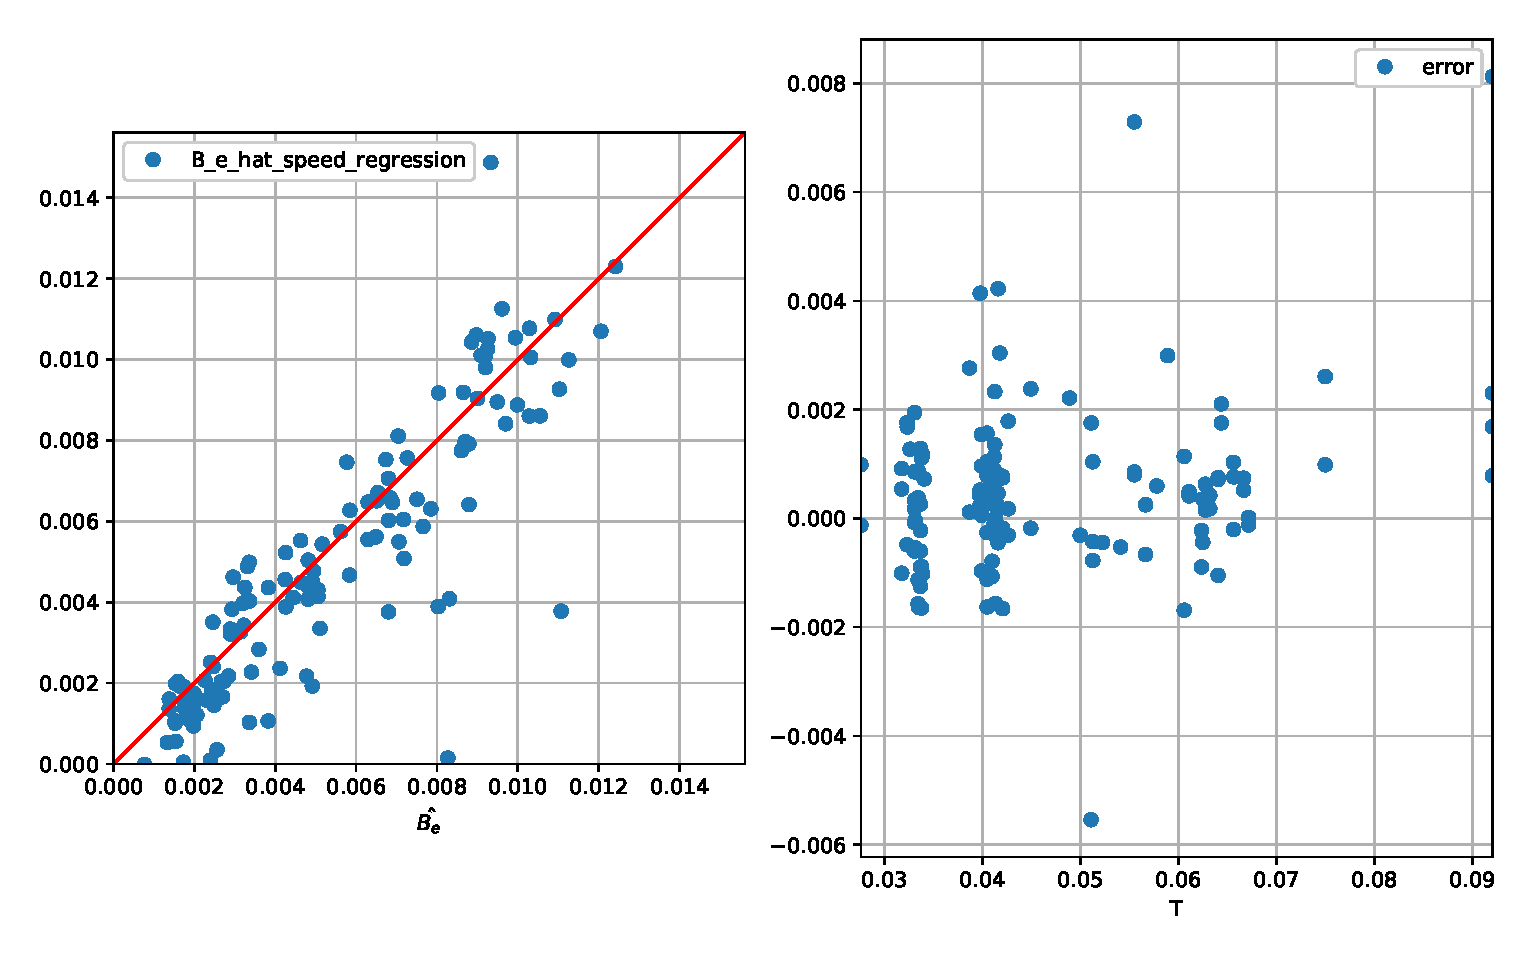
\includegraphics[width=\columnwidth]{figures/B_e_factor_regression_total.eps}
    \caption{Total regression}
    \label{fig:B_e_factor_regression_total}
\end{figure}

\section{Conclusions}
\label{se:conclusions}
The roll damping database has been compared with predictions with the implementation of the Simplified Ikeda method. The database and the predictions show agreement for some cases but poor agreement for other cases, especially for small draft to beam ratios, typically for Ballast loading condition for many modern ships. It seems that exceeding the limits of the the Simplified Ikeda method will give poor results. These limits are unfortunately not so well defined in \parencite{kawahara_simple_2011}. The comparison in the present paper suggest a lower limit of the draught to length ratio of $T/L_{pp}>0.034$.

A regression model has been developed which has better accuracy than the Simplified method for the present roll damping data. The accuracy of the regression model has been investigated using extensive cross validation. The model should be able to predict the roll damping for ships with main dimensions similar to the once in this paper within the estimated accuracy.
If higher accuracy is needed, more advanced methods can be used, such as the original Ikeda method with strip calculations, CFD or model testing, to get reliable roll damping predictions.

\section{Discussion}
The test setup in the free roll decay tests differs from the forced roll motion model tests that Ikeda \parencite{ikeda_velocity_1979} used to derive the original method. This is not believed to have any large impact as long as roll damping near the natural frequency is considered. The Ikeda model tests were also conducted with smaller models (2 meters compared to 3-6 meters). But there is a skin friction component $B_F$ to the Ikeda method that should handle this scale effect.



\section*{Acknowledgements}
\label{se:acknowledgements}
The authors would like to acknowledge Trafikverket (Swedish Transport Administration) and Lighthouse for providing the resources to prepare this paper and also thank all personnel at SSPA that have been involved in the creation of the model test results: building the ship models and conducting the experiments. Also special thanks to Sune Thorsson who collected the meta data about the tested ship models.






%\begin{appendices}

\appendix
\section{Ship models}\label{app:ships}
\begin{figure}[H]
    \centering
    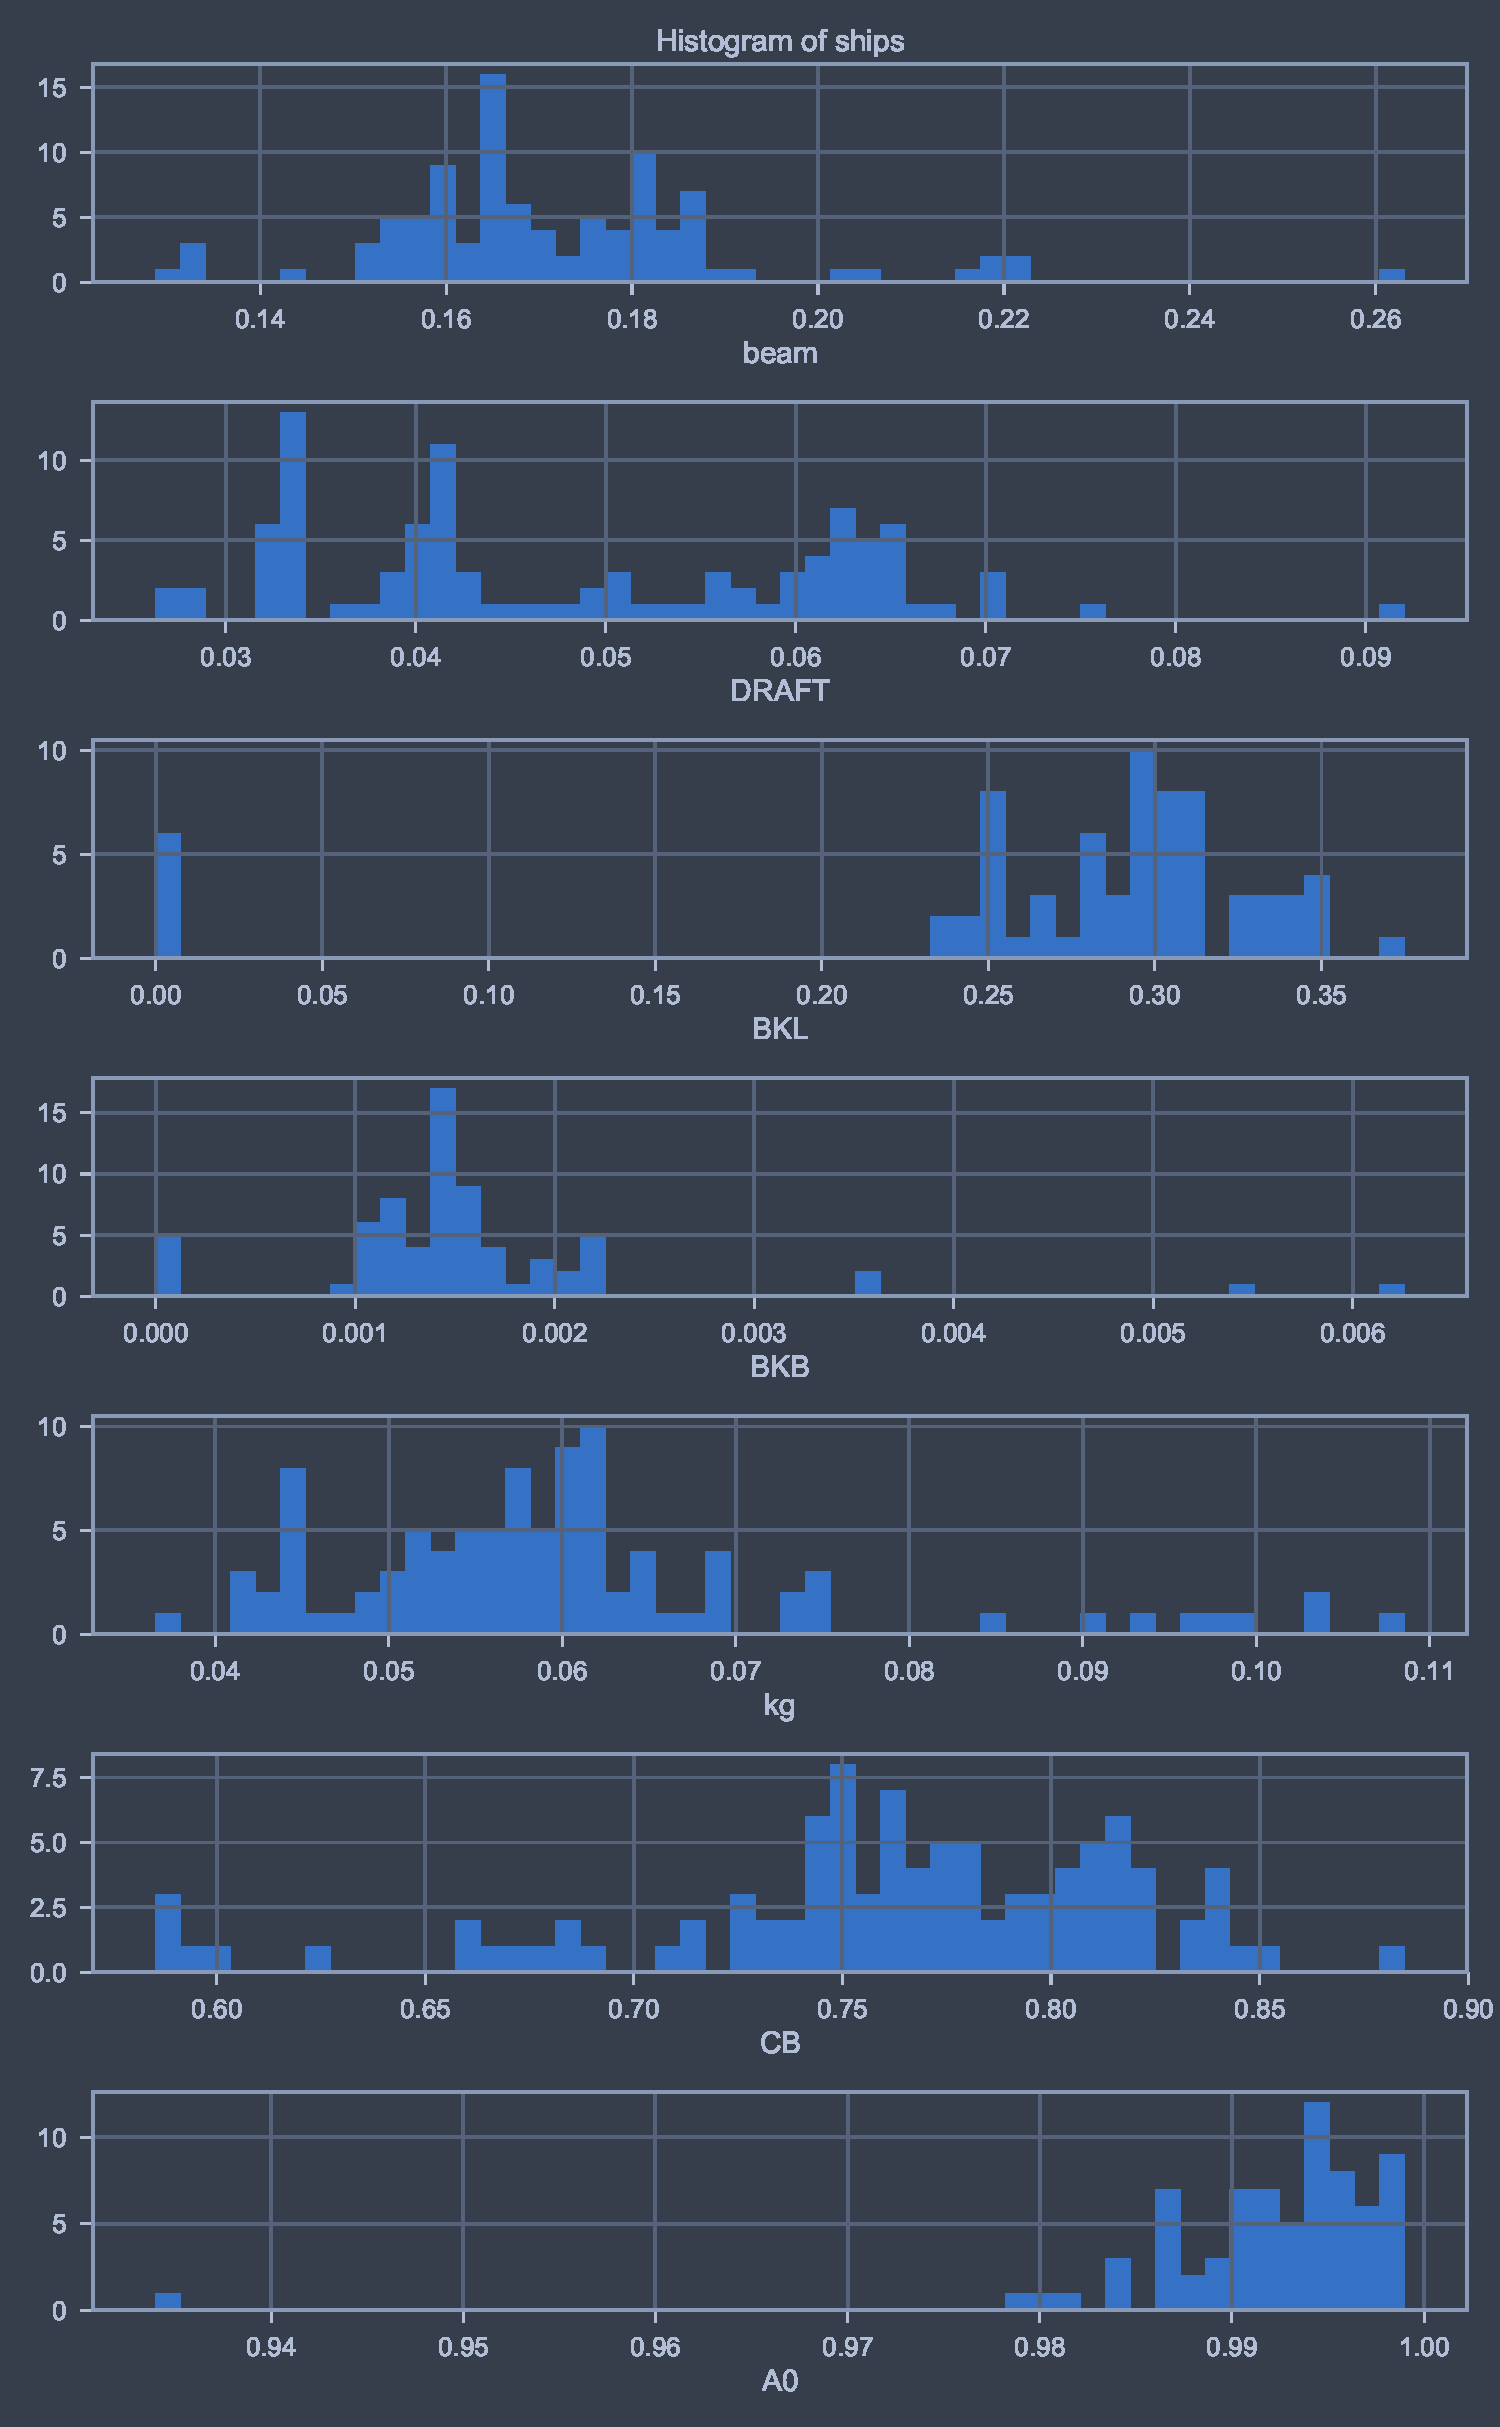
\includegraphics[width=0.7\columnwidth]{figures/ship_parameters.pdf}
    \caption{Histograms of ship parameters from the model tests, all parameters except CB and A0 have been normalized with Lpp}
    \label{fig:ship_parameters}
\end{figure}

\begin{figure}[H]
    \centering
    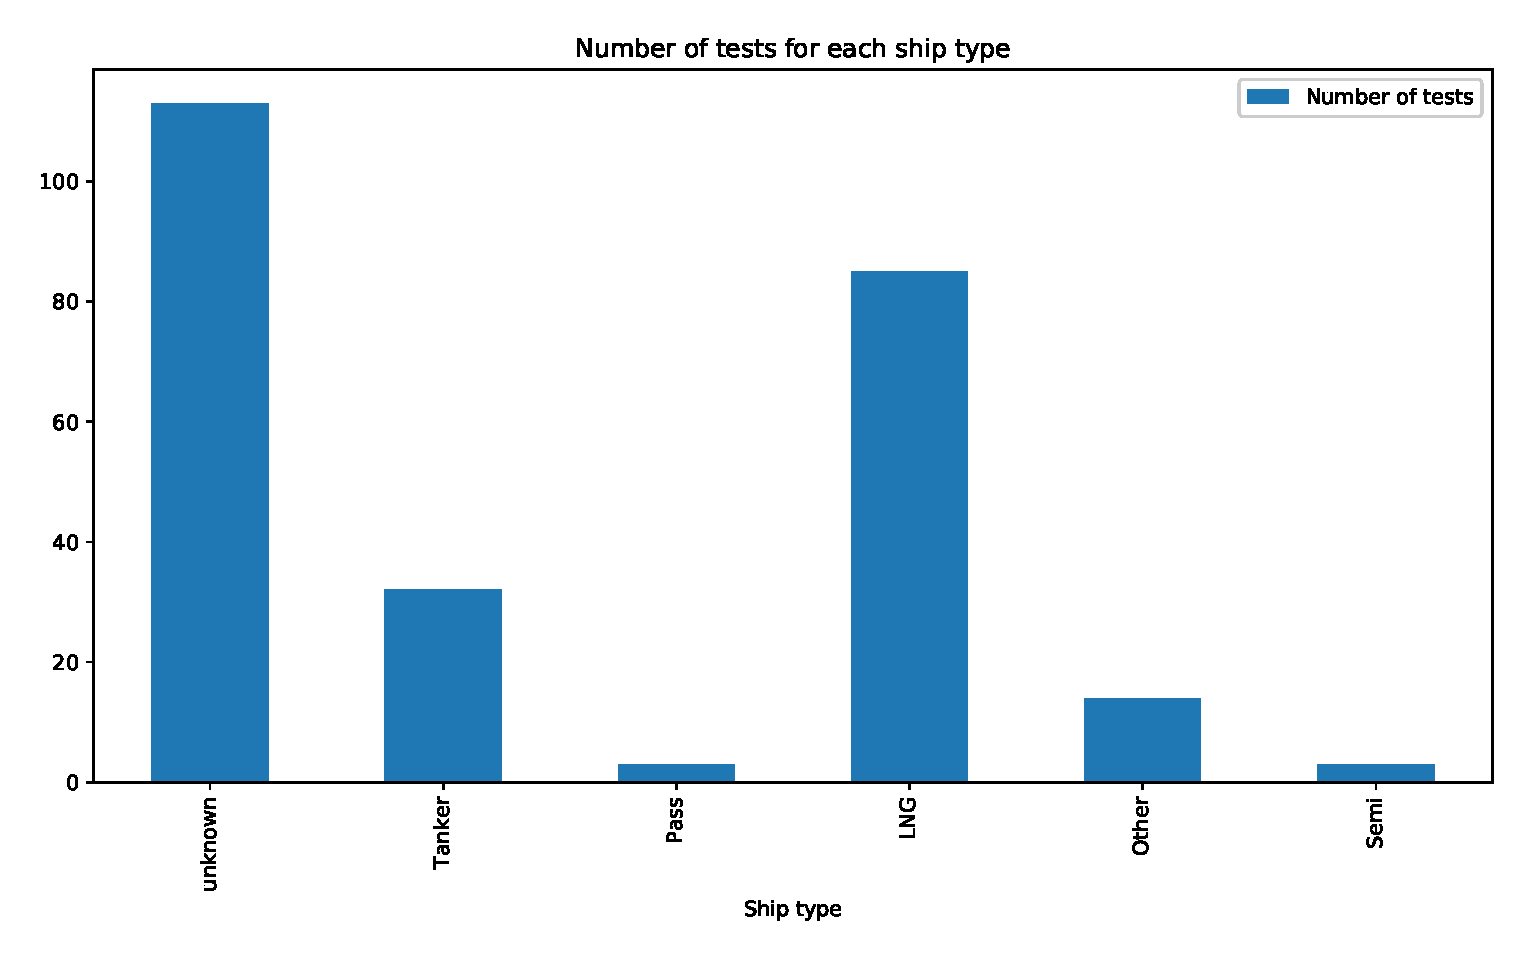
\includegraphics[width=0.7\columnwidth]{figures/ship_types.eps}
    \caption{Number of tests per ship type}
    \label{fig:ship_types}
\end{figure}


%\end{appendices}
\section{References}
\label{sec:references}

\bibliographystyle{unsrt}
%\bibliographystyle{abbrvnat}
\bibliography{references}


\end{document}
